\subsubsection{Completed Three-Group Factorial}

All 24 logical F models, their three readouts and seven-view scoring are complete. The 12 missing combinations were newly trained; the other 12 weights and eligible predictions were reused. Independent local aggregation recomputed 24192 serialized confusion matrices, same-F raw agreement and paired repair/damage nets. The five complete CSVs agree numerically across Python versions (maximum absolute difference $9.95\times10^{-14}$, tolerance $10^{-10}$). Table~\ref{tab:core-complete} reports the predeclared four primary rows; Fig.~\ref{fig:core-full} retains every factorial cell. All error bars and $\pm$ values are sample SD over the three F seeds, conditional on each fixed G.

\begin{table*}[t]\centering\footnotesize

\caption{Completed primary F ablation (Accuracy, \%). Six-scene means are formed within seed first. The fixed G-L and G-LU are distinct training-data conditions.}\label{tab:core-complete}

\begin{tabular}{clcccc}\toprule ABC & Setting & Raw clean & Raw six scenes & G-L six scenes & G-LU six scenes\\\midrule

111 & Full T1 & $84.394\pm0.916$ & $70.601\pm1.062$ & $76.703\pm0.969$ & $77.647\pm0.846$\\

011 & Without A: CRIC & $84.728\pm0.506$ & $70.990\pm1.238$ & $77.037\pm0.557$ & $78.057\pm0.485$\\

101 & Without B: paired consistency & $83.141\pm0.761$ & $70.498\pm0.613$ & $75.534\pm0.431$ & $76.635\pm0.480$\\

110 & Without C: selective SSL & $84.785\pm0.824$ & $70.596\pm0.952$ & $76.854\pm0.592$ & $77.855\pm0.396$\\

\bottomrule\end{tabular}\end{table*}

\begin{figure*}[t]\centering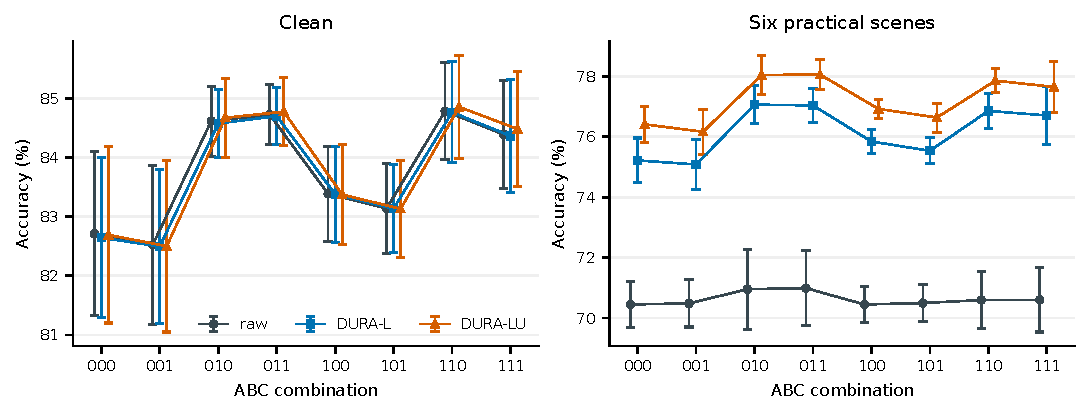
\includegraphics[width=\textwidth]{images/core/core_factorial_accuracy.pdf}

\caption{All eight predeclared ABC combinations, three F seeds per cell, with raw/G-L/G-LU readouts. C=0 plus G-L is L-only; attaching G-LU uses U through G. These are not three independently replicated complete systems.}\label{fig:core-full}\end{figure*}

The conditional group effects are full 111 minus the corresponding removal, paired by F seed (Table~\ref{tab:core-effects} and Fig.~\ref{fig:core-removals}). B improves raw clean accuracy by $1.2534\pm1.0933$ points, with positive differences in all three seeds. Its raw six-scene effect is only $0.1033\pm0.5171$ points (two positive seeds), while its G-LU six-scene effect is $1.0119\pm0.8031$ points (three positive seeds).

In contrast, A and C do not show a consistent positive contribution in the full combination: their raw clean effects are $-0.3331\pm0.8420$ and $-0.3909\pm0.7248$ points, respectively, with only one positive seed each. Their G-LU six-scene effects are also negative on average. These results do not support claiming that all three groups provide stable gains under this fixed F0 condition. They are retained without changing the designated default, regrouping components or selecting reruns from target scores.

\begin{table}[t]\centering\footnotesize\setlength{\tabcolsep}{3pt}

\caption{Full-minus-removal paired Accuracy differences (points).}\label{tab:core-effects}

\begin{tabular}{cccc}\toprule Group & Raw clean & Raw six & G-LU six\\\midrule

A & $-0.333\pm0.842$ & $-0.388\pm1.223$ & $-0.411\pm0.384$\\

B & $1.253\pm1.093$ & $0.103\pm0.517$ & $1.012\pm0.803$\\

C & $-0.391\pm0.725$ & $0.005\pm0.716$ & $-0.208\pm0.582$\\

\bottomrule\end{tabular}\end{table}

\begin{figure*}[t]\centering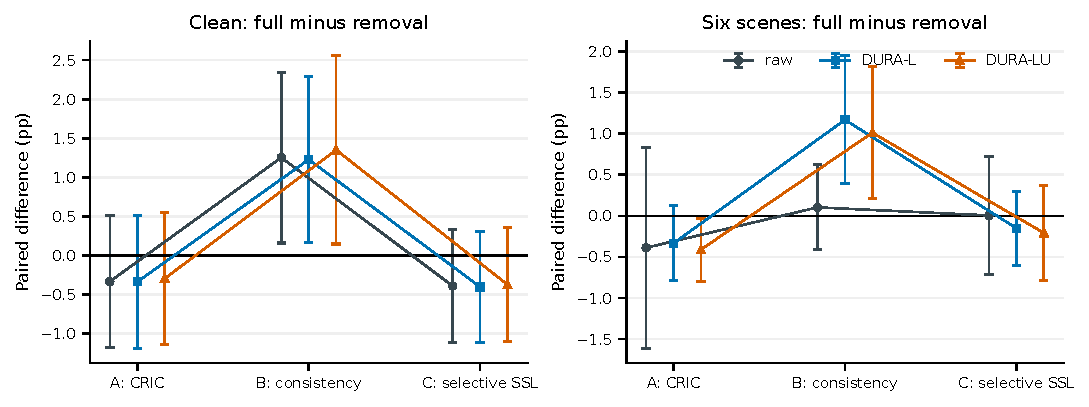
\includegraphics[width=\textwidth]{images/core/core_leave_one_group_out.pdf}

\caption{Seed-paired full-minus-removal differences. The zero line and all negative effects are retained; sample SD does not constitute a significance test.}\label{fig:core-removals}\end{figure*}

The complete factorial distinguishes conditional effects from marginal averages. On raw clean data, the A/B/C effects averaged over the other switches are $0.2812\pm0.4464$, $1.6904\pm0.7742$, $-0.1794\pm0.2147$ points. A therefore has different marginal and full-model conditional directions. The AB clean interaction, averaged over C, is $-0.7288\pm0.6185$ points (negative in all three seeds). Raw six-scene AB interaction is $-0.3799\pm0.4214$ points. Fig.~\ref{fig:core-interactions} reports all interactions; no additive contribution or general benefit is inferred from isolated cells.

\begin{figure}[t]\centering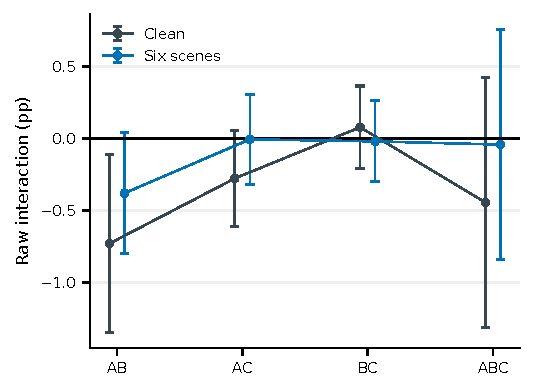
\includegraphics[width=\columnwidth]{images/core/core_raw_interactions.pdf}

\caption{Raw interaction contrasts, mean$\pm$sample SD over F seeds. AB/AC/BC are difference-in-differences averaged over the remaining switch; ABC is the signed eight-cell contrast.}\label{fig:core-interactions}\end{figure}

For full T1, G-L improves the six-scene mean over raw by $6.1020\pm0.3396$ points; G-LU adds $0.9436\pm0.2730$ points over G-L. The G-LU/raw total is the already reported F0 result, not new independent replication. C-off/G-LU is not a fully supervised system. Per-scene/RX/TX/date Accuracy, Macro-F1 and repair/damage counts are preserved in the frozen results.

\paragraph{Source-only physical diagnostics.} All 24 F weights use the same 720 labeled source observations from 90 TX/RX/day strata, with at most eight per stratum. No U, target data or fitted diagnostic classifier is accessed. Same-day anchor-balanced cosine distances separate same-TX cross-RX pairs from different-TX same-RX pairs. Full T1 gives same-TX cross-RX distance $0.0618\pm0.0105$, versus $0.0685\pm0.0118$ without A. However, its different-TX separation margin does not increase (Fig.~\ref{fig:core-geometry}). Lower within-identity distance alone does not establish full receiver/channel invariance or better target identification.

\begin{figure*}[t]\centering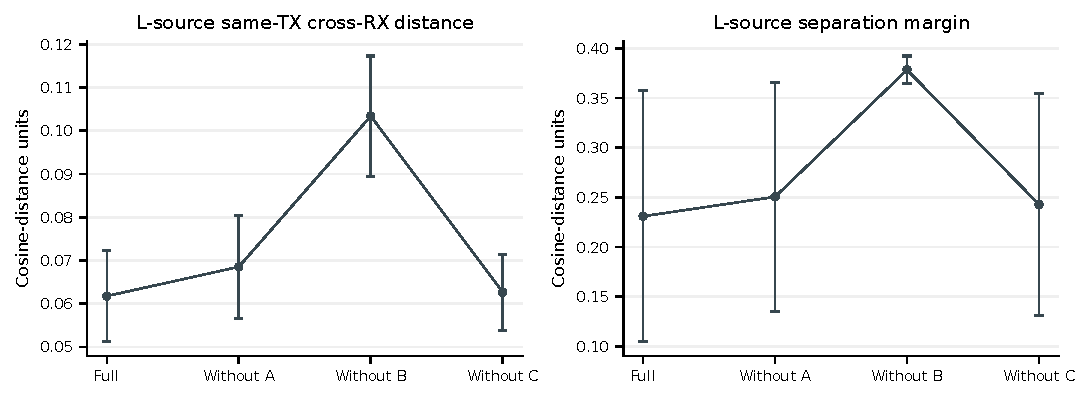
\includegraphics[width=\textwidth]{images/core/core_source_geometry.pdf}

\caption{Paired source-L geometry of the four primary settings. Separation margin is different-TX/same-RX distance minus same-TX/cross-RX distance. This descriptive analysis does not fit a new head or establish hardware disentanglement.}\label{fig:core-geometry}\end{figure*}

Eleven fixed interventions cover identity, flat gain, constant phase, relative CFO, FIR echo and simulated PA. Feature cosine distance, default-head prediction flips and reference-descriptor relative error are retained for every setting. Simulated PA changes are not assumed identity preserving. These diagnostics provide controlled sensitivity evidence; the independently trained physical-structure panel remains pending.

\paragraph{Actual incremental cost.} The 12 new F models use 600 model-epochs/133200 updates and sum to 20.453 shared-worker elapsed hours. All 24 logical F sources, including reused T1 segments, sum to 40.623 hours under differing historical contention; this is not the additional cost of this extension or exclusive GPU time. No G or separate classification head is trained here; G ancestor costs remain separate. A/B/C change training objectives, not the deployed graph, so no unmeasured per-ablation latency is inferred from the completed default timing panel.
